% Toy paper for the AI for Research seminar.
%
% Illustrative only. This skeleton is meant to be filled in by an AI agent
% working from the Stack Overflow Annual Developer Survey data.
% See ../README.md for the workflow.

\documentclass[11pt]{article}

\usepackage[a4paper, margin=2.5cm]{geometry}
\usepackage{graphicx}
\usepackage{booktabs}
\usepackage{amsmath}
\usepackage{hyperref}
\usepackage{natbib}
\usepackage{authblk}

\title{AI-tool adoption and self-reported job satisfaction among professional
software developers: a descriptive analysis of the Stack Overflow Annual
Developer Survey}

\author[1]{Author One}
\author[1]{Author Two}
\affil[1]{Universidade Cat\'olica Portuguesa}

\date{\today}

\begin{document}
\maketitle

\begin{abstract}
We use the 2025 Stack Overflow Annual Developer Survey to describe the
relationship between professional developers' reported adoption of AI coding
tools and their reported job satisfaction, controlling for years of
professional work experience and primary developer role. In a complete-case
sample of 24,354 respondents, daily reported AI-tool use is associated with
job satisfaction that is 0.16--0.22 points higher on a 0--10 scale than
non-use, conditional on experience and role ($p<0.001$). The association is
not monotonic across use-intensity categories, and the full model explains
under two percent of the variance in satisfaction. The analysis is
descriptive only: the survey is observational, selection into the sample is
not random, and both the regressor and the outcome are self-reported on the
same instrument. We discuss in detail why these features rule out a causal
or even a confidently generalizable reading of the result. This paper is a
teaching artefact produced for a seminar on AI for research; it is not
intended for publication and should not be cited as evidence that AI tools
improve (or harm) developer satisfaction.
\end{abstract}

\section{Introduction}

Whether the rapid adoption of AI coding assistants is good for the developers
who use them is a question with obvious practical stakes: for tool vendors
deciding what to build, for managers deciding what to mandate, and for
developers deciding what to learn. The Stack Overflow Annual Developer
Survey offers a tempting shortcut to an empirical answer, because it asks
tens of thousands of professional developers, in the same instrument, both
how often they use AI tools and how satisfied they are with their job.

We use this opportunity to ask a narrow, descriptive question: among
survey respondents, is self-reported AI-tool adoption associated with
self-reported job satisfaction, after conditioning on years of professional
experience and primary developer role? We want to be explicit from the
outset about what this question is not. It is not a causal question, and
the data cannot answer one. The survey is a single cross-section of
self-selected respondents who self-report both variables on the same
instrument; there is no experimental or quasi-experimental source of
variation in AI-tool adoption, and no way to rule out reverse causality
(satisfied developers may be more willing to experiment with new tools)
or common confounders (employer policy, team culture, individual ability)
that plausibly drive both adoption and satisfaction.

Our contribution is accordingly not a substantive finding but a transparent,
fully reproducible worked example: a complete pipeline from a public,
licensed dataset, through descriptive statistics and a pre-registered-style
regression specification, to a written paper that states its own limits
as carefully as it states its results. This paper was produced for a
seminar on AI tools for research, and its main pedagogical point is
contained as much in Section~\ref{sec:limitations} as in Section~\ref{sec:results}:
an honest descriptive analysis of an opportunistic online survey should
report a small, fragile association and say so plainly, rather than dress
it up as evidence of an effect.

\section{Data}

We use the 2025 wave of the Stack Overflow Annual Developer Survey
\citep{stackoverflow2025survey}, a voluntary, self-administered online
survey of software developers and other technology professionals,
fielded by Stack Overflow and advertised primarily to registered users of
the Stack Overflow website and associated channels. The survey is released
under the Open Database License (ODbL) 1.0 for the database structure and
the Database Contents License (DbCL) 1.0 for the cell contents; both permit
sharing and derivative use with attribution. The raw file contains
49{,}191 respondents and 172 columns covering demographics, employment,
technology use, and attitudes toward AI tools.

We construct four analysis variables. \emph{AI-tool use} is taken from the
survey item \texttt{AISelect}, which asks how often the respondent uses AI
tools in their development workflow, with response categories ``daily,''
``weekly,'' ``monthly or infrequently,'' ``no, but plan to,'' and ``no, and
do not plan to.'' For our primary specification we collapse this into a
binary indicator equal to 1 for any current use (daily, weekly, or
monthly/infrequent) and 0 for no current use (whether or not the respondent
plans to start); a secondary specification retains the original five
categories to check for a dose-response pattern. \emph{Job satisfaction}
is the survey's derived \texttt{JobSat} score, a 0--10 index built by
Stack Overflow from a battery of point-allocation items
(\texttt{JobSatPoints\_1}--\texttt{16}) asking respondents to distribute
points across sources of job satisfaction; we use the index as supplied.
\emph{Years of professional experience} is \texttt{WorkExp}, self-reported
years of professional work experience (this year's instrument does not
field a separate ``years coding professionally'' item, so this is the
closest available measure). \emph{Primary developer role} is
\texttt{DevType}, a 32-category self-classification; to keep a
fixed-effects specification tractable we retain the ten most frequent
categories (full-stack, back-end, student, architect, front-end,
desktop/enterprise, mobile, embedded, academic researcher, and an explicit
``other, please specify'' write-in option) and group all remaining
categories into a residual ``Other'' bucket.

Missingness differs sharply across these four variables: 31.5\% on
\texttt{AISelect}, 45.8\% on \texttt{JobSat}, 12.8\% on \texttt{WorkExp},
and 11.2\% on \texttt{DevType}. \texttt{JobSat} is by far the largest
source of attrition. Our analysis sample keeps only respondents with
non-missing values on all four variables simultaneously, giving
$N = 24{,}354$, or 49.5\% of the raw 49{,}191 respondents. We return to
the consequences of this large, and possibly non-random, drop in
Section~\ref{sec:limitations}. In the analysis sample, job satisfaction
averages 7.22 (SD 1.98, median 8, on the 0--10 scale) and professional
experience averages 13.6 years (SD 10.1, median 11); 80.8\% of the
analysis sample (19,680 of 24,354) reports current AI-tool use of some
frequency.

\section{Method}

We estimate two ordinary least squares specifications, both with
heteroskedasticity-robust (HC1) standard errors and developer-role fixed
effects. The primary specification is
\begin{equation}
  \mathrm{JobSat}_i = \beta_0 + \beta_1\, \mathrm{AIUser}_i + \beta_2\, \mathrm{WorkExp}_i
  + \sum_k \gamma_k\, \mathrm{DevType}_{ik} + \varepsilon_i,
  \label{eq:m1}
\end{equation}
where $\mathrm{AIUser}_i$ is the binary current-use indicator described
above. The secondary specification replaces $\mathrm{AIUser}_i$ with four
dummy variables for the original use-intensity categories (``plan to soon,''
``monthly/infrequent,'' ``weekly,'' ``daily''), with ``no, and do not plan
to'' as the reference category, to check whether any association is
concentrated in heavy users or spread evenly across any reported use.

The implicit hypothesis we are testing is $H_0: \beta_1 = 0$ (no
conditional association between reported AI-tool adoption and reported job
satisfaction) against $H_1: \beta_1 \neq 0$. Tech-industry discourse around
AI coding assistants typically motivates a one-sided expectation that
$\beta_1 > 0$ (tools that remove drudgery should raise satisfaction), but
we test two-sided, since a negative association (frustration with imperfect
tools, anxiety about deskilling) is equally easy to motivate ex ante.

We want to flag the interpretive status of $\beta_1$ before presenting any
numbers. Equation~\eqref{eq:m1} is a conditional correlation, not an effect.
\texttt{AIUser} is not assigned to respondents by anything resembling
random variation; it reflects respondents' own choices, made for reasons
(employer policy, curiosity, perceived skill threats, existing workload)
that are not captured by the two controls we include. Whatever sign and
magnitude $\hat\beta_1$ takes, it should be read as ``developers who
report using AI tools also report different satisfaction, net of experience
and role,'' not as ``using AI tools changes satisfaction.''

\section{Results}
\label{sec:results}

\subsection{Descriptive statistics}

Table~\ref{tab:descriptives} reports unconditional mean, median, and
standard deviation of job satisfaction by reported AI-tool use, before any
adjustment for experience or role. Mean satisfaction is similar across the
non-use and light-use categories (7.11--7.14) and highest among daily
users (7.29). Figure~\ref{fig:sat-by-ai} plots the same means with
standard-error bars and shows that the gap between daily users and every
other category, while real, is small relative to the spread of the
satisfaction scale itself (SD $\approx 2$ points in every group).

\begin{table}[h]
\centering
\caption{Job satisfaction (0--10) by reported AI-tool use, full sample with
non-missing \texttt{JobSat}.}
\label{tab:descriptives}
\begin{tabular}{lrrrr}
\toprule
AI-tool use & $N$ & Mean & Median & SD \\
\midrule
No, and do not plan to              & 3{,}643  & 7.14 & 8.0 & 2.12 \\
No, but plan to soon                & 1{,}135  & 7.11 & 8.0 & 2.08 \\
Yes, monthly or infrequently        & 3{,}188  & 7.11 & 7.0 & 2.02 \\
Yes, weekly                         & 4{,}353  & 7.14 & 7.0 & 1.89 \\
Yes, daily                          & 12{,}599 & 7.29 & 8.0 & 1.96 \\
\bottomrule
\end{tabular}
\end{table}

\begin{figure}[h]
  \centering
  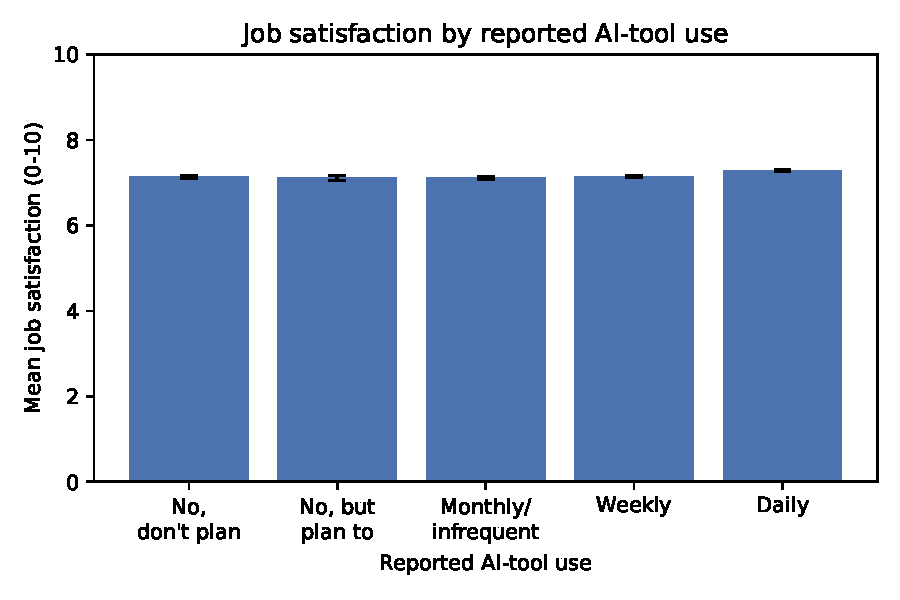
\includegraphics[width=0.8\linewidth]{figures/fig1_satisfaction_by_ai_use.pdf}
  \caption{Mean self-reported job satisfaction by reported AI-tool use,
  with standard-error bars. Full sample with non-missing \texttt{JobSat}
  ($N = 24{,}918$ across the five categories shown).}
  \label{fig:sat-by-ai}
\end{figure}

A descriptive fact that matters for interpreting the regression below:
reported AI-tool use is not evenly distributed across experience levels.
In the same data, mean professional experience is 12.8 years among daily
users and 13.5--14.8 years among weekly and monthly/infrequent users, but
16.2--18.5 years among respondents who do not currently use AI tools.
Less experienced developers are systematically more likely to report
using AI tools, which is exactly why we condition on \texttt{WorkExp} in
the regression rather than reading the raw means in
Table~\ref{tab:descriptives} on their own. Figure~\ref{fig:years} shows
the distribution of professional experience in the analysis sample: it is
right-skewed, with a median of 11 years, an interquartile range of 6--20
years, and a long tail (the maximum recorded value, 100 years, is almost
certainly a data-entry or top-coding artifact rather than a literal
century of work experience).

\begin{figure}[h]
  \centering
  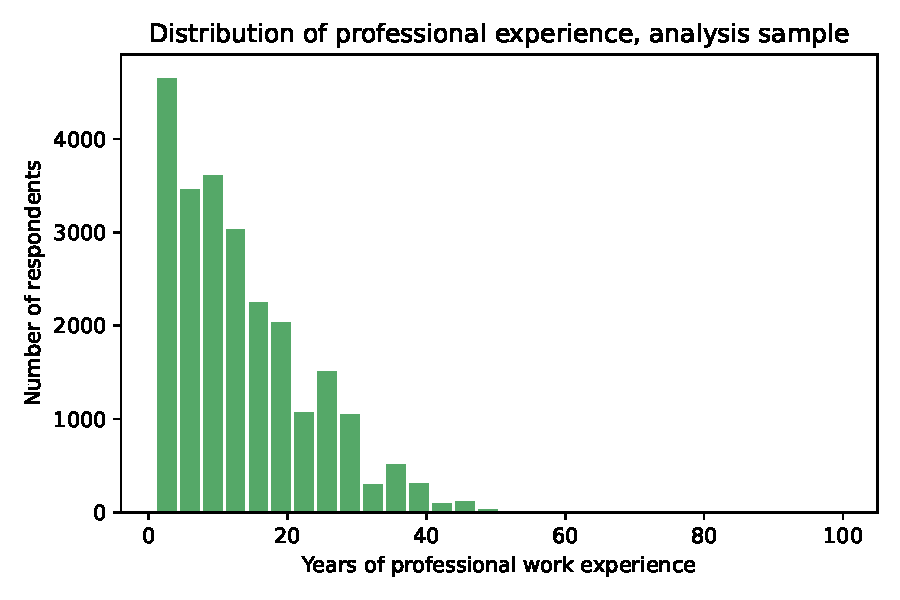
\includegraphics[width=0.8\linewidth]{figures/fig2_years_experience.pdf}
  \caption{Distribution of years of professional work experience
  (\texttt{WorkExp}) in the analysis sample ($N = 24{,}354$).}
  \label{fig:years}
\end{figure}

\subsection{Regression results}

Table~\ref{tab:regression} reports the two specifications. In Model 1, the
binary AI-use indicator has a coefficient of 0.164 (HC1 SE 0.034,
$p < 0.001$): conditional on professional experience and developer role,
current AI-tool users report job satisfaction 0.16 points higher, on the
0--10 scale, than non-users. We can reject $H_0: \beta_1 = 0$ at any
conventional significance level. Years of professional experience also
carries a small positive, highly significant coefficient (0.021 points per
year, $p < 0.001$).

Model 2 disaggregates AI-tool use by intensity. Relative to respondents who
do not currently use AI tools and do not plan to, daily users report
satisfaction 0.221 points higher ($p < 0.001$); weekly users 0.065 points
higher (not distinguishable from zero, $p = 0.154$); monthly/infrequent
users 0.009 points higher (indistinguishable from zero, $p = 0.861$); and
respondents who plan to start using AI tools soon report satisfaction
0.058 points \emph{lower} (also indistinguishable from zero, $p = 0.409$).
The association in Model 1 is therefore not a smooth dose-response
relationship: it is driven almost entirely by the daily-use subgroup, while
occasional use is statistically indistinguishable from non-use.

\begin{table}[h]
\centering
\caption{OLS regressions of job satisfaction (0--10) on AI-tool use,
years of professional experience, and developer-role fixed effects.
Heteroskedasticity-robust (HC1) standard errors in parentheses.}
\label{tab:regression}
\begin{tabular}{lcc}
\toprule
 & Model 1 & Model 2 \\
\midrule
AI user (vs.\ non-user)            & 0.164$^{***}$ (0.034) & --- \\
\quad No, but plan to soon         & --- & $-$0.058 (0.071) \\
\quad Yes, monthly/infrequent      & --- & 0.009 (0.050) \\
\quad Yes, weekly                  & --- & 0.065 (0.046) \\
\quad Yes, daily                   & --- & 0.221$^{***}$ (0.040) \\
Years of professional experience   & 0.021$^{***}$ (0.001) & 0.021$^{***}$ (0.001) \\
\midrule
Developer-role fixed effects       & Yes (10 categories + Other) & Yes (10 categories + Other) \\
$N$                                 & 24{,}354 & 24{,}354 \\
$R^2$                               & 0.016 & 0.018 \\
\bottomrule
\end{tabular}

\medskip
\noindent\footnotesize $^{*}p<0.05$, $^{**}p<0.01$, $^{***}p<0.001$. Reference category
for AI-use dummies in Model 2 is ``no, and do not plan to.'' Full
developer-role coefficients (reference category: academic researcher) are
reported in the project's replication files; in both models the largest
and most precisely estimated role coefficients are negative for back-end
($-0.44$, $p<0.001$) and front-end ($-0.42$, $p<0.001$) developers relative
to academic researchers, with full-stack, mobile, desktop/enterprise, and
embedded developers in between.
\normalsize
\end{table}

Two features of these results matter as much as the statistically
significant coefficients themselves. First, both models explain very
little of the variation in job satisfaction: $R^2 = 0.016$ and $0.018$
respectively, meaning AI-tool use, experience, and developer role jointly
account for under two percent of why respondents differ in reported
satisfaction. Second, the coefficient sizes are small relative to the
spread of the outcome: a 0.164--0.221 point shift on a 0--10 scale with a
sample standard deviation near 2.0 corresponds to a standardized effect
(Cohen's $d$) of roughly 0.08 to 0.11 -- below the conventional threshold
for even a ``small'' effect. With $N$ in the tens of thousands, coefficients
this small are still easy to distinguish statistically from zero; that is
a reminder that, in large samples, statistical significance is not a
proxy for practical importance.

\section{Limitations}
\label{sec:limitations}

We treat this section as the headline of the paper, not a footnote, because
every limitation below applies with full force to the numbers just
reported.

\textbf{Selection into the survey.} Respondents are not a probability
sample of professional developers worldwide. They are people who use Stack
Overflow, saw the survey invitation, and chose to spend roughly twenty
minutes completing it. This selects on platform engagement, English-language
fluency or comfort, geography (our sample's top countries are the United
States, Germany, India, the United Kingdom, and France), and plausibly on
attitudes toward both surveys and technology adoption. Nothing in our
analysis corrects for this; the results describe \emph{respondents to this
survey}, not developers in general.

\textbf{Selection into the analysis sample.} Half of the raw respondents
are dropped because they are missing at least one of our four variables,
overwhelmingly because they skipped or were not shown the job-satisfaction
items (45.8\% missing on \texttt{JobSat} alone). If non-response on job
satisfaction is itself correlated with job satisfaction or with AI-tool
use -- which is entirely plausible (e.g., dissatisfied respondents skipping
a multi-part satisfaction battery, or respondents who skip optional content
also being less engaged with newer tools) -- our complete-case sample is a
further, unquantified, non-random subset of an already non-random survey.

\textbf{Self-report on both sides of the regression, from the same
instrument.} AI-tool use and job satisfaction are both self-reported in
the same survey, by the same respondent, in the same sitting. This invites
common-method variance: respondents with a generally positive (or
acquiescent) response style may report both more frequent tool use and
higher satisfaction for reasons that have nothing to do with any real
relationship between the two. We have no second, independent measure of
either variable to check against.

\textbf{No identification strategy for AI-tool adoption.} \texttt{AISelect}
is not assigned by anything resembling random variation. Adoption is
plausibly endogenous to factors we cannot observe in this survey: individual
ability and curiosity, employer policy and tooling budgets, team norms,
and -- most importantly for our specific question -- job satisfaction
itself. Reverse causality is at least as plausible as the causal story
implicit in the research question: a developer who is already satisfied
and engaged may be more willing to experiment with new tools, rather than
new tools making developers more satisfied. Our regression cannot
distinguish these stories, and no amount of additional control variables
in a single cross-section would fix this; the fix is a different design
(panel data with within-person variation, an instrument for adoption, or
a field experiment), not available here.

\textbf{Omitted variables.} We condition on experience and role only.
Employer, compensation, management quality, team culture, and the
specific tasks a respondent's job involves are all plausible confounders
that we do not observe well enough to control for (compensation, where
available, is itself over 50\% missing and extremely heavy-tailed).

\textbf{Cross-sectional, single wave.} We use one year of one survey. We
cannot speak to trends, cannot use any respondent as their own control
before and after adopting AI tools, and cannot say whether the small
association we find is stable or specific to this particular year's
labor-market and tooling conditions.

\textbf{Measurement and replicability of the underlying instrument.} The
survey instrument itself changes from year to year -- this year's wave
retired the ``years of professional coding experience'' item used in
earlier waves of this same survey in favor of a more general ``years of
professional work experience'' item, which is why our experience control
is not identical in definition to the variable used in past analyses of
this survey. Replicating this analysis on a different year's file requires
re-checking the codebook, not simply re-running the same code.

\textbf{Practical magnitude.} As noted in Section~\ref{sec:results}, the
full model explains under two percent of the variance in job satisfaction,
and the AI-use coefficients correspond to effect sizes well below
conventional thresholds for a ``small'' effect. Even if every other
limitation above were resolved, the substantive size of this association
would not support strong claims either way about AI tools and developer
well-being.

In short: this is opportunistic, observational, self-reported survey data,
with substantial and likely non-random attrition, no design that
identifies a causal pathway, and a result whose statistical significance
is a function of sample size more than of effect size. None of this means
the descriptive numbers are wrong; it means they should not be asked to
carry more interpretive weight than ``in this self-selected sample of
Stack Overflow survey respondents, daily AI-tool users reported very
slightly higher job satisfaction than non-users, net of experience and
role.''

\section{Conclusion}

We documented a small, statistically significant, but practically modest
positive association between reported daily AI-tool use and reported job
satisfaction among respondents to the 2025 Stack Overflow Developer Survey,
conditional on years of professional experience and developer role. The
association is concentrated in daily users specifically; weekly and
occasional use are statistically indistinguishable from non-use, and the
full specification accounts for under two percent of the variance in
satisfaction. We found no evidence of a negative association between
AI-tool adoption and satisfaction, but we also found no evidence strong
enough, or designed well enough, to support a causal claim in either
direction. Selection into the survey, selection into the analysis sample,
shared-method self-report on both variables, and the absence of any
source of independent variation in AI-tool adoption are, jointly, more
important to take away from this paper than the regression coefficients.

This paper is a teaching artefact for a seminar on AI tools for research,
not a contribution to the literature on AI adoption and worker well-being.
Its purpose was to demonstrate, end to end, a reproducible pipeline from a
public licensed dataset to descriptive statistics, a regression
specification, and a written, appropriately hedged set of conclusions --
and, just as importantly, to show what it looks like when that pipeline is
used honestly: a small effect, reported as small, in a sample whose limits
are stated as plainly as its results.

\bibliographystyle{plainnat}
\bibliography{refs}

\end{document}
